\documentclass[12pt,a4paper]{article}
\usepackage{ctex}
\usepackage{amsmath}
\usepackage{algorithmic} 
\usepackage{amssymb}
\usepackage{graphicx}
\usepackage{booktabs}
\usepackage{geometry}
\usepackage{float}
\usepackage{subcaption}
\usepackage{listings}
\usepackage{hyperref}

\geometry{a4paper,left=2.5cm,right=2.5cm,top=2.5cm,bottom=2.5cm}

\title{行星际飞行轨道递推计算与分析}
\author{xxx}
\date{\today}

\begin{document}

\maketitle

\begin{abstract}
    本实验报告深入探讨了行星际飞行轨道递推计算与分析,旨在通过构建日心坐标系和火心坐标系下的轨道动力学模型,运用 \textbf{Kepler 方程解析解法} 和 \textbf{四阶 Runge-Kutta 数值积分方法},实现对行星际探测器轨道的精准递推。研究核心聚焦于不同轨道递推方法的精度对比、火星引力辅助变轨的偏转效果以及长期轨道预测的可行性。

    在 \textbf{Kepler 轨道递推} 过程中,引入了选择判断机制,以优化步长设计。实验发现,固定步长虽能提升计算效率,但可能导致运动遗漏,降低精度。为此,提出在大部分时间点采用较大步长提高效率,而在最后一个时间点动态调整步长至剩余时间增量,以确保精度。这种动态调整策略有效平衡了效率与精度,避免了因截止时间残余而导致的运动遗漏。

    在 \textbf{双曲线 Kepler 轨道递推} 方面,针对火星引力辅助变轨,详细分析了探测器在火星引力作用下的轨道特性。双曲线轨道的偏心率 e > 1,轨道能量为正值,探测器在引力场中做双曲线运动。通过牛顿迭代法求解双曲线轨道的 Kepler 方程,实现了轨道根数到位置和速度矢量的转换。实验结果表明,探测器在火星引力作用下发生了显著的轨道偏转,速度和角动量均发生了显著变化,轨道能量增加,成功实现了轨道调整。

    实验最终绘制了日心坐标系下探测器、火星和地球的飞行轨道图,直观展示了探测器的运动轨迹及其与行星的相对位置关系。该轨道图在任务规划、轨道控制和科学研究中具有重要价值,为深空探测任务的实施提供了有力支持。报告成功验证了不同轨道递推方法的可行性和有效性,为行星际探测任务的轨道设计与优化提供了重要参考。本实验所有源代码均已开源于\url{https://github.com/LiuZiyue1016/Keplerian-Motion}。
\end{abstract}

\textbf{关键词:行星际飞行 ; Kepler 轨道递推 ; 数值积分 ; 火星引力辅助变轨 ; 轨道预测}

\section{问题提出}
本实验通过建立日心坐标系和火心坐标系下的轨道动力学模型,分别采用Kepler方程解析解法和四阶Runge-Kutta数值积分方法实现行星际探测器的轨道递推计算。重点研究:
\begin{itemize}
    \item 不同轨道递推方法的精度比较
    \item 火星引力辅助变轨的偏转效果
    \item 长期轨道预测的可行性分析
\end{itemize}

\section{实验任务与参数}
\subsection{给定参数}
太阳、火星引力常数:
\begin{equation*}
    \begin{aligned}
        \mu_{\text{sun}} &= 1.32712440017987 \times 10^{11}\ \mathrm{km^3/s^2} \\
        \mu_{\text{mars}} &= 4.28283762065 \times 10^{4}\ \mathrm{km^3/s^2}
    \end{aligned}
\end{equation*}

地球在$t_0$时刻的日心初始位置和速度矢量:
\begin{equation*}
    \begin{aligned}
        \mathbf{r}_{\text{earth}} &=
        \begin{bmatrix}
             0.110937729685236 \\
             1.346867468212425 \\
             0.583831802330196
        \end{bmatrix}
        \times 10^8
        \ \mathrm{km} \\
        \mathbf{v}_{\text{earth}} &= 
        \begin{bmatrix}
            -30.200703848645549 \\
            1.956654058695767\\
            0.847099469360955
        \end{bmatrix}\ \mathrm{km/s}
    \end{aligned}
\end{equation*}

探测器在$t_0$时刻的日心初始位置和速度矢量:
\begin{equation*}
    \begin{aligned}
        \mathbf{r}_0 &=
        \begin{bmatrix}
            -0.370264 \\ 
            1.315142 \\ 
            0.608323
        \end{bmatrix}
        \times 10^8
        \ \mathrm{km} \\
        \mathbf{v}_0 &= 
        \begin{bmatrix}
            -31.80621 \\ 
            -6.234824 \\ 
            -0.078191
        \end{bmatrix}\ \mathrm{km/s}
    \end{aligned}
\end{equation*}

火星在探测器到达火星时的日心位置和速度矢量:
\begin{equation*}
    \begin{aligned}
        \mathbf{r}_{\text{Mars}} &=
        \begin{bmatrix}
            0.598177 \\ 
            -1.853298 \\ 
            -0.866201
        \end{bmatrix}
        \times 10^8
        \ \mathrm{km} \\
        \mathbf{v}_{\text{Mars}} &= 
        \begin{bmatrix}
            24.16545 \\ 
            8.313188 \\ 
            3.161448
        \end{bmatrix}\ \mathrm{km/s}
    \end{aligned}
\end{equation*}

时间参数:
\begin{equation*}
    \begin{aligned}
        t_1 &= 279.1318\ \text{天} \quad (\text{探测器从$t_0$时刻飞行至火星影响球时间}) \\        
        t_2 &= 3.83448\ \text{天} \quad (\text{探测器飞进到飞出火星影响球内时间}) \\
        t_3 &= 500\ \text{天} \quad (\text{探测器飞出火星引力影响球后的飞行时间})
    \end{aligned}
\end{equation*}

\subsection{任务流程}
\begin{enumerate}
    \item 日心坐标系Kepler轨道递推($t_1$)
    \item 日心坐标系数值积分轨道递推($t_1$)
    \item Keplar和数值积分轨道递推对比
    \item 火心坐标系数值积分轨道递推($t_2$)
    \item 偏转效果定量分析
    \item 日心坐标系keplar轨道递推($t_3$)
    \item 绘制日心和火心探测器轨道飞行图及地球、火星飞行轨道图
\end{enumerate}

\section{基础理论与实现}
\subsection{Kepler轨道递推}

已知某物体绕中心天体作椭圆运动,$t_0$时刻的位置和速度矢量为$\mathbf{r}_0$和$\mathbf{v}_0$,试求$t$时刻的位置和速度矢量$\mathbf{r}(t)$和$\mathbf{v}(t)$。

计算步骤:
\begin{enumerate}
    \item 将初始位置和速度矢量$\mathbf{r}_0$和$\mathbf{v}_0$转化为轨道六根数:
    $$
    x_0 = \left[a, e, i, \Omega, \omega, E_0\right]
    $$
    
    \item 根据偏近点角$E_0$和开普勒方程计算平近点角$M_0$;
    
    \item 由轨道平均运动计算$t$时刻平近点角:
    $$
    M(t) = M_0 + n(t - t_0)
    $$
    
    \item 迭代求解开普勒方程获得$t$时刻偏近点角$E(t)$    \item 将新的轨道根数转化为$t$时刻的位置和速度矢量$\mathbf{r}(t)$和$\mathbf{v}(t)$。
\end{enumerate}

\begin{figure}[H]
    \centering
    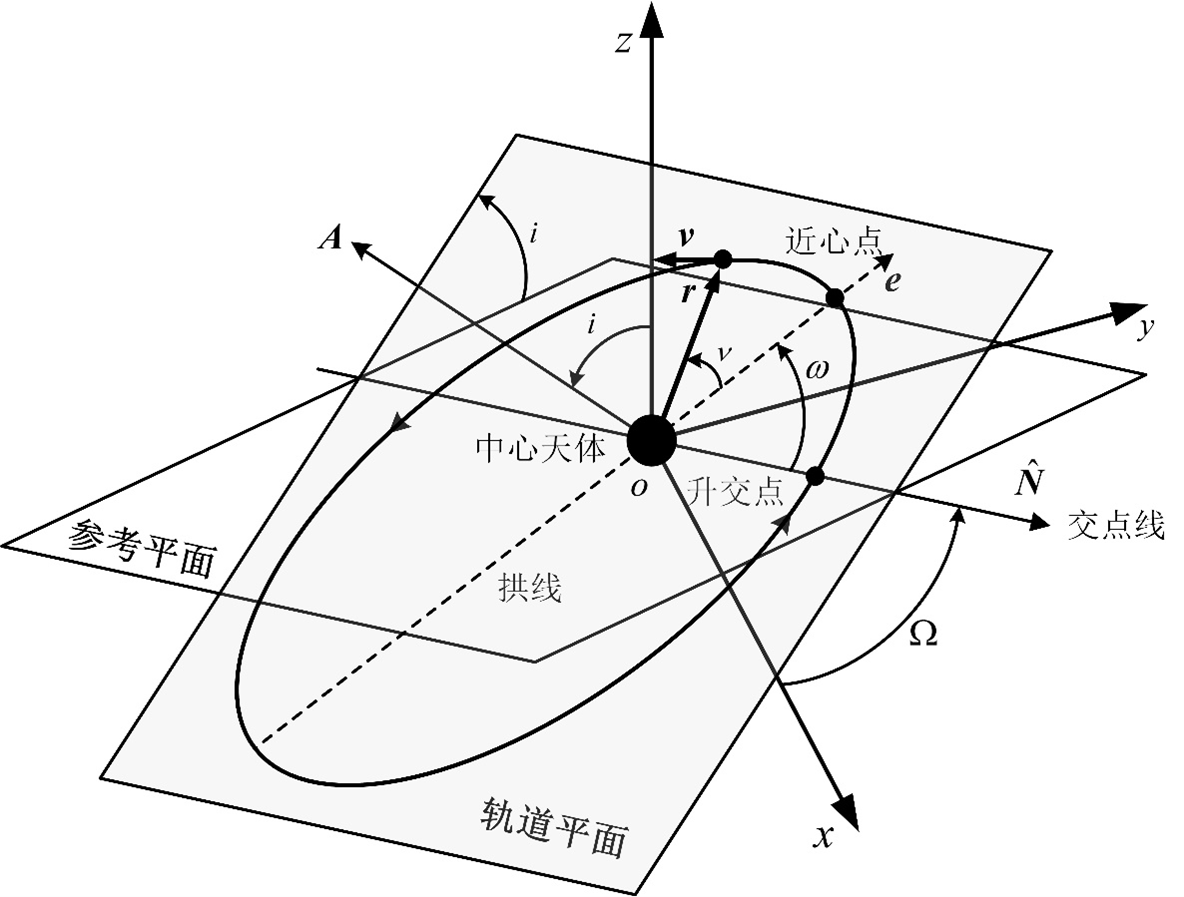
\includegraphics[width=0.8\textwidth]{images/coe.png}
    \caption{轨道六根数}
\end{figure}

\lstinputlisting[language=Matlab]{code/kepler_propagate.m}

\subsection{轨道六根数和位置速度矢量的相互转化}
\subsubsection{位置和速度矢量转轨道六根数}

已知轨道位置矢量$\mathbf{r}$和速度矢量$\mathbf{v}$,可唯一确定轨道六根数。在参考惯性坐标系中,角动量矢量表示为:
$$
\mathbf{A} = \begin{bmatrix} A_x \\ A_y \\ A_z \end{bmatrix} = \mathbf{r} \times \mathbf{v} = \begin{bmatrix} y\dot{z} - z\dot{y} \\ z\dot{x} - x\dot{z} \\ x\dot{y} - y\dot{x} \end{bmatrix}
$$
根据轨道根数的定义,角动量矢量亦可表示为:
$$
\mathbf{A} = A \begin{bmatrix} \sin i \sin\Omega \\ -\sin i \cos\Omega \\ \cos i \end{bmatrix}
$$
联立上式可得轨道倾角和升交点赤经:
\begin{equation}
i = \arccos\left( \frac{A_z}{A} \right)
\end{equation}
\begin{equation}
\Omega = \arctan 2\left( \frac{A_x}{A \sin i}, -\frac{A_y}{A \sin i} \right)
\end{equation}

轨道半长轴表示为:
$$
a = \left( \frac{2}{r} - \frac{v^2}{\mu} \right)^{-1}
$$
轨道半通径和偏心率分别为:
\begin{equation}
p = \frac{A^2}{\mu} = a(1 - e^2)
\end{equation}
\begin{equation}
e = \sqrt{1 - \frac{p}{a}}
\end{equation}

平均角速度为:
$$
n = \sqrt{\frac{\mu}{|a|^3}}
$$

椭圆轨道几何关系:
$$
\mathbf{r} \cdot \mathbf{v} = \sqrt{\mu a} \frac{a e \sin E}{r}(1 - e \cos E)
$$
结合$r = a(1 - e \cos E)$可得:
$$
\mathbf{r} \cdot \dot{\mathbf{r}} = a^2 n e \sin E
$$
解得:
\begin{equation}
\sin E = \frac{\mathbf{r} \cdot \mathbf{v}}{a^2 n e}, \quad \cos E = \frac{a - r}{a e}
\end{equation}

真近点角关系:
$$
\begin{cases}
\cos v = \dfrac{\cos E - e}{1 - e \cos E} \\
\sin v = \dfrac{\sqrt{1 - e^2} \sin E}{1 - e \cos E}
\end{cases}
$$

纬度幅角$u = \omega + v$满足:
$$
\begin{cases}
r \cos u = x \cos\Omega + y \sin\Omega \\
r \sin u = \dfrac{z}{\sin i}
\end{cases}
$$
解得近地点幅角:
$$
\omega = u - v
$$

\lstinputlisting[language=Matlab]{code/rv2coe.m}

\subsubsection{轨道六根数转位置和速度矢量}

近焦点坐标系中位置矢量为:
$$
\mathbf{r}_e = r \begin{bmatrix} \cos v \\ \sin v \\ 0 \end{bmatrix}
$$
转换矩阵为:
$$
M_e = R_z(-\Omega) R_x(-i) R_z(-\omega)
$$
其中旋转矩阵:
$$
R_x(\phi) = \begin{bmatrix}
1 & 0 & 0 \\
0 & \cos\phi & \sin\phi \\
0 & -\sin\phi & \cos\phi
\end{bmatrix}, \quad
R_z(\phi) = \begin{bmatrix}
\cos\phi & \sin\phi & 0 \\
-\sin\phi & \cos\phi & 0 \\
0 & 0 & 1
\end{bmatrix}
$$

惯性坐标系中位置矢量:
$$
\mathbf{r} = M_e \mathbf{r}_e = r \cos v \hat{\mathbf{s}}_x + r \sin v \hat{\mathbf{s}}_y
$$
单位矢量:
$$
\hat{\mathbf{s}}_x = \begin{bmatrix}
\cos\omega \cos\Omega - \sin\omega \cos i \sin\Omega \\
\cos\omega \sin\Omega + \sin\omega \cos i \cos\Omega \\
\sin\omega \sin i
\end{bmatrix}, \quad
\hat{\mathbf{s}}_y = \begin{bmatrix}
-\sin\omega \cos\Omega - \cos\omega \cos i \sin\Omega \\
-\sin\omega \sin\Omega + \cos\omega \cos i \cos\Omega \\
\cos\omega \sin i
\end{bmatrix}
$$

速度矢量:
$$
\mathbf{v} = \frac{\sqrt{\mu a}}{r} \left[ -\sin E \hat{\mathbf{s}}_x + \sqrt{1 - e^2} \cos E \hat{\mathbf{s}}_y \right]
$$

\lstinputlisting[language=Matlab]{code/coe2rv.m}

\subsection{Kepler方程的求解}

椭圆轨道Kepler方程:
\begin{equation}
E - e \sin E = M
\end{equation}

定义辅助函数:
$$
f(E) = E - e \sin E - M
$$
其导数为:
$$
\frac{df}{dE} = 1 - e \cos E > 0
$$
牛顿迭代公式:
$$
E_{k+1} = E_k - \frac{f(E_k)}{1 - e \cos E_k}
$$
迭代至收敛精度$\varepsilon$满足。

\lstinputlisting[language=Matlab]{code/solve_kepler.m}

\subsection{ode45数值积分轨道递推}
ode45 是一种基于自适应步长的 Runge-Kutta 方法,结合了四阶和五阶公式,用于求解常微分方程(ODE)。它的核心思想是通过误差估计自动调整步长,以在满足精度要求的同时提高计算效率。

ode45 的公式基于以下 Runge-Kutta 方法:
\[
\begin{cases}
\mathbf{y}_{n+1} = \mathbf{y}_n + h \sum_{i=1}^6 b_i \mathbf{k}_i \\
\mathbf{k}_1 = f(t_n, \mathbf{y}_n) \\
\mathbf{k}_2 = f\left(t_n + c_2 h, \mathbf{y}_n + h \sum_{j=1}^1 a_{2j} \mathbf{k}_j\right) \\
\mathbf{k}_3 = f\left(t_n + c_3 h, \mathbf{y}_n + h \sum_{j=1}^2 a_{3j} \mathbf{k}_j\right) \\
\mathbf{k}_4 = f\left(t_n + c_4 h, \mathbf{y}_n + h \sum_{j=1}^3 a_{4j} \mathbf{k}_j\right) \\
\mathbf{k}_5 = f\left(t_n + c_5 h, \mathbf{y}_n + h \sum_{j=1}^4 a_{5j} \mathbf{k}_j\right) \\
\mathbf{k}_6 = f\left(t_n + c_6 h, \mathbf{y}_n + h \sum_{j=1}^5 a_{6j} \mathbf{k}_j\right)
\end{cases}
\]
其中,\(h\) 是当前步长,\(f(t, \mathbf{y})\) 是状态向量的导数函数,\(c_i, a_{ij}, b_i\) 是方法的系数。

ode45 使用五阶公式计算下一步的解,并用四阶公式估计误差,根据误差估计,步长 \(h\) 会被动态调整以满足用户设定的容差。
\[
\begin{cases}
\mathbf{y}_{n+1}^{(5)} = \mathbf{y}_n + h \sum_{i=1}^6 b_i \mathbf{k}_i \\
\mathbf{y}_{n+1}^{(4)} = \mathbf{y}_n + h \sum_{i=1}^5 \tilde{b}_i \mathbf{k}_i \\
\text{误差估计:} \quad \text{err} = \left|\mathbf{y}_{n+1}^{(5)} - \mathbf{y}_{n+1}^{(4)}\right|
\end{cases}
\]

在轨道动力学中,状态向量通常包含位置和速度分量。对于三维空间中的天体运动,状态向量可以表示为:
\[
\mathbf{y} = \begin{bmatrix}
x & y & z & \dot{x} & \dot{y} & \dot{z}
\end{bmatrix} ^ {T}
\]
其中,\(x, y, z\) 是位置分量,\(\dot{x}, \dot{y}, \dot{z}\) 是速度分量。

状态向量的导数由牛顿运动定律和引力公式给出:
\[
\frac{d\mathbf{y}}{dt} = \begin{bmatrix}
\dot{x} & \dot{y} & \dot{z} & a_x & a_y & a_z
\end{bmatrix} ^ {T}
\]
其中,\(a_x, a_y, a_z\) 是引力加速度分量,由牛顿万有引力公式计算:
\[
a_x = -\frac{\mu x}{r^3}, \quad a_y = -\frac{\mu y}{r^3}, \quad a_z = -\frac{\mu z}{r^3}
\]
其中,\(\mu = GM\) 是引力参数,\(G\) 是引力常数,\(M\) 是中心天体的质量,\(r = \sqrt{x^2 + y^2 + z^2}\) 是位置向量的模长。

\lstinputlisting[language=Matlab]{code/sun_gravity.m}

\section{实现结果与分析}
\subsection{轨道递推探测器状态}

在具体实验中,我们设计 Kepler 递推的步长为 100,牛顿迭代的容忍度为 \(10^{-10}\)。实验表明,Kepler 递推的步长对其精度影响较小,但步长设计是收集轨道数据的必然操作。然而,由于截止时间包含残余时间,在收集轨道状态数据时会遗漏这些时间的运动,导致 Kepler 递推的精度下降。

为解决这一问题,我们引入选择判断机制:首先将数据扩展一个长度,当递推至倒数第一个数据时,将步长从原有值动态调整为剩余的所有时间。这种方法既考虑了剩余时间的运动,又通过增大步长提高了效率。

以下是 Kepler 递推步长的动态调整算法:

\begin{algorithm}
\caption{Kepler 递推步长动态调整}
\begin{algorithmic}
\FOR{$j = 1$ to $n_{\text{time}} - 1$}
    \IF{$j == n_{\text{time}} - 1$}
        \STATE 计算剩余时间增量:
        \[
        dt_{\text{step}} = t(j+1) - t(j)
        \]
    \ELSE
        \STATE 使用固定步长:
        \[
        dt_{\text{step}} = dt
        \]
    \ENDIF
    \STATE 使用 \(dt_{\text{step}}\) 计算下一个时间点的平近点角
\ENDFOR
\end{algorithmic}
\end{algorithm}

设总时间为 \(T\),时间步长为 \(dt\),时间点序列为 \(t_0, t_1, \dots, t_{n_{\text{time}}}\),其中 \(t_0 = 0\),\(t_{n_{\text{time}}} = T\)。在 Kepler 递推中,平近点角 \(M\) 的计算公式为:
\[
M_{j+1} = M_j + {dt_{\text{step}}}n
\]
其中 \(n\) 为平均角速度。

当步长固定为 \(dt\) 时,时间点序列为:
\[
t_j = t_0 + j \cdot dt
\]
但由于截止时间 \(T\) 可能包含残余时间 \(\Delta t = T - t_{n_{\text{time}}}\),最后一个时间点的步长需要调整为:
\[
dt_{\text{step}} = \Delta t
\]

通过动态调整步长,我们可以在效率和精度之间取得平衡:
\begin{itemize}
    \item 当步长较大时(如 \(dt = 100\)),计算复杂度为 \(O(n_{\text{time}})\),效率较高,但可能遗漏部分运动。
    \item 当步长较小时(如 \(dt = 1\)),计算复杂度为 \(O(n_{\text{time}} \cdot dt)\),精度较高,但效率较低。
    \item 通过动态调整步长,我们可以在大部分时间点使用较大步长以提高效率,而在最后一个时间点使用剩余时间增量以保证精度。
\end{itemize}


\subsubsection{到达火星影响球时的日心轨道状态}
\begin{itemize}
    \item \textbf{Kepler 方法计算结果}:
    \begin{itemize}
        \item 位置: 
        \[
        \begin{bmatrix}
            60361624.824665 \\ -185410365.859250 \\ -86444351.414516
        \end{bmatrix} \, \text{km}
        \]
        \item 速度:         
        \[
        \begin{bmatrix}
            20.952597 \\ 8.763759 \\ 2.095795
        \end{bmatrix} \, \text{km/s}
        \]
    \end{itemize}
    
    \item \textbf{数值积分方法计算结果}:
    \begin{itemize}
        \item 位置: 
        \[
        \begin{bmatrix}
            60361624.826628 \\ -185410365.858303 \\ -86444351.414275
        \end{bmatrix} \, \text{km}
        \]
        \item 速度: 
        \[
        \begin{bmatrix}
            20.952597 \\ 8.763759 \\ 2.095795
        \end{bmatrix} \, \text{km/s}
        \]
    \end{itemize}
    
    \item \textbf{两种方法的偏差}:
    \begin{itemize}
        \item 位置偏差: 
        \[
        \begin{bmatrix}
            -0.001963 \\ -0.000947 \\ -0.000241
        \end{bmatrix} \, \text{km}
        \]
        \item 速度偏差: 
        \[
        \begin{bmatrix}
            0.000000 \\ -0.000000 \\ -0.000000
        \end{bmatrix} \, \text{km/s}
        \]
    \end{itemize}
\end{itemize}

\subsubsection{Kepler 方法预测的后续轨道状态}
\begin{itemize}
    \item \textbf{飞出火星引力影响球 500 天后的日心轨道状态}:
    \begin{itemize}
        \item 位置: 
        \[
        \begin{bmatrix}
            -171953401.842335 \\ -167965202.830318 \\ -76448722.227815
        \end{bmatrix} \, \text{km}
        \]
        \item 速度: 
        \[
        \begin{bmatrix}
            16.413362 \\ -11.536247 \\ -5.498273
        \end{bmatrix} \, \text{km/s}
        \]
    \end{itemize}
\end{itemize}

\subsection{火星借力偏转轨道}
与椭圆轨道不同,双曲线轨道的偏心率 \(e > 1\),轨道能量为正值,探测器在引力场中做双曲线运动。双曲线轨道的推导需要使用双曲函数代替椭圆轨道中的三角函数,同时轨道根数的计算和轨道方程的形式也有所不同。

\subsubsection{双曲线kepler轨道递推}
双曲线轨道的径向距离公式为:
\begin{equation}
    r = \frac{p}{1 + e \cos(\theta)}
\end{equation}
其中:
- \(p = a(1 - e^2)\) 是半参数;
- \(a < 0\) 是半长轴;
- \(e > 1\) 是偏心率;
- \(\theta\) 是真近点角。

由于 \(e > 1\),分母 \(1 + e \cos(\theta)\) 可能为零或负值,因此需要确保 \(\theta\) 的范围使得分母为正值。

双曲线轨道的平均角速度 \(n\) 定义为:
\begin{equation}
    n = \sqrt{\frac{\mu}{(-a)^3}}
\end{equation}
其中 \(\mu\) 是引力参数,\(-a\) 是半长轴的绝对值。

双曲线轨道的平近点角 \(M\) 和偏近点角 \(F\) 的关系为:
\begin{equation}
    M = e \sinh(F) - F
\end{equation}
其中 \(\sinh(F)\) 是双曲正弦函数。

偏近点角 \(F\) 和真近点角 \(\theta\) 的关系为:
\begin{equation}
    \tan\left(\frac{\theta}{2}\right) = \sqrt{\frac{e + 1}{e - 1}} \tanh\left(\frac{F}{2}\right)
\end{equation}

双曲线轨道的 Kepler 方程为:
\begin{equation}
    M = e \sinh(F) - F
\end{equation}
由于无法直接求解 \(F\),需要使用数值方法(如牛顿迭代法)来求解。

牛顿迭代法的步骤如下:
1. 初始猜测 \(F_0 = M\);
2. 迭代公式:
   \begin{equation}
       F_{k+1} = F_k - \frac{e \sinh(F_k) - F_k - M}{e \cosh(F_k) - 1}
   \end{equation}
3. 当 \(|F_{k+1} - F_k| < \text{tol}\) 时停止迭代。

将轨道根数转换为位置和速度向量时,双曲线轨道的公式与椭圆轨道不同:
- 径向距离:
  \begin{equation}
      r = \frac{p}{1 + e \cos(\theta)}
  \end{equation}
- 速度向量:
  \begin{equation}
      \mathbf{v} = \sqrt{\frac{\mu}{p}} \left[ -\sin(\theta), \, e + \cos(\theta), \, 0 \right]^T
  \end{equation}

与椭圆轨道相比,双曲线轨道具有以下特性:
- 轨道能量为正值;
- 探测器在引力场中做双曲线运动,最终逃离引力场;
- 轨道六根数转换位置速度中使用双曲函数代替三角函數。

\lstinputlisting[language=Matlab]{code/hyperbolic_kepler_propagate.m}

\lstinputlisting[language=Matlab]{code/solve_kepler_hyperbola.m}

\subsubsection{探测器飞入火星影响球时的轨道状态(通过双曲线 Kepler 轨道递推)}
\begin{itemize}
    \item 位置: 
    \[
    \begin{bmatrix}
        543895.109373 \\ -80552.648235 \\ 175744.755863
    \end{bmatrix} \, \text{km}
    \]
    \item 半径: \(577232.048964 \, \text{km}\)
    \item 速度矢量: 
    \[
    \begin{bmatrix}
        -3.212852 \\ 0.450571 \\ -1.065653
    \end{bmatrix} \, \text{km/s}
    \]
    \item 速度: \(3.414828 \, \text{km/s}\)
\end{itemize}

\subsubsection{探测器飞出火星影响球时的轨道状态(通过双曲线 Kepler 轨道递推)}
\begin{itemize}
    \item 位置: 
    \[
    \begin{bmatrix}
        -334568.929582 \\ 390148.928996 \\ 262762.510256
    \end{bmatrix} \, \text{km}
    \]
    \item 半径: \(577231.922395 \, \text{km}\)
    \item 速度矢量: 
    \[
    \begin{bmatrix}
        -1.951262 \\ 2.316482 \\ 1.577193
    \end{bmatrix} \, \text{km/s}
    \]
    \item 速度: \(3.414828 \, \text{km/s}\)
\end{itemize}

\subsubsection{效果分析}

探测器飞越火星时的双曲线轨道参数满足:
\begin{equation}
    v_p = \sqrt{v_{\infty}^2 + \frac{2\mu}{r_p}}
\end{equation}
其中$\mu = \mu_{\text{mars}}$, $r_p$为近火点距离,$v_{\infty}$为无限远处相对速度。

速度矢量叠加关系(质心系):
\begin{align}
    \mathbf{V}^- &= \mathbf{v}_{\text{mars}} + \mathbf{v}_{\infty}^- \\
    \mathbf{V}^+ &= \mathbf{v}_{\text{mars}} + \mathbf{v}_{\infty}^+
\end{align}

速度改变量模长:
\begin{equation}
    \Delta v = 2v_{\infty} \sin\left(\frac{\delta}{2}\right)
\end{equation}

其中偏转角$\delta$由下式确定:
\begin{equation}
    \tan\left(\frac{\delta}{2}\right) = \frac{\mu}{r_p v_{\infty}^2}
\end{equation}

在质心惯性坐标系中,探测器的角动量可以表示为:
\begin{equation}
    H = \|\mathbf{R} \times \mathbf{v}\| = X_1 \dot{Y}_1 - Y_1 \dot{X}_1
\end{equation}

质心惯性坐标系中探测器借力飞行前后的轨道能量变化量为:
\begin{equation}
    \Delta E = -2 v_2 v_{\infty} \sin \frac{\delta}{2} \sin \psi
\end{equation}

\begin{figure}[H]
    \centering
    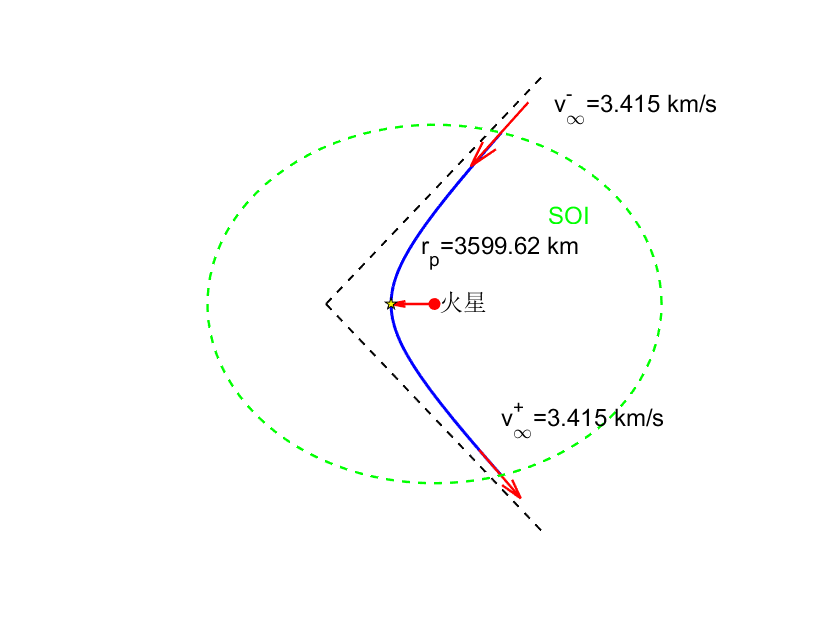
\includegraphics[width=0.8\textwidth]{images/schematic.png}
    \caption{火星借力飞行轨道示意图}
\end{figure}

\begin{table}[H]
    \centering
    \caption{火星引力偏转效果参数表}
    \label{tab:mars_gravity}
    \begin{tabular}{lc}
        \toprule
        指标 & 数值 \\
        \midrule
        近地点半径$r_p$ & $3604.196629\,\mathrm{km}$ \\
        借力飞行高度 & 
        $214.996629\,\mathrm{km}$\\
        角动量变化$\Delta H$ & $5.3185 \times 10^{8}\,\mathrm{km^{2}/s}$ \\
        速度增量$\Delta v$ & $3.4724\,\mathrm{km/s}$ \\
        偏转角$\delta$ & $61.1194^\circ$ \\
        轨道能量变化$\Delta E$ & $-65.2349\,\mathrm{km^2/s^2}$ \\
        \bottomrule
    \end{tabular}
\end{table}

\begin{figure}[H]
    \centering
    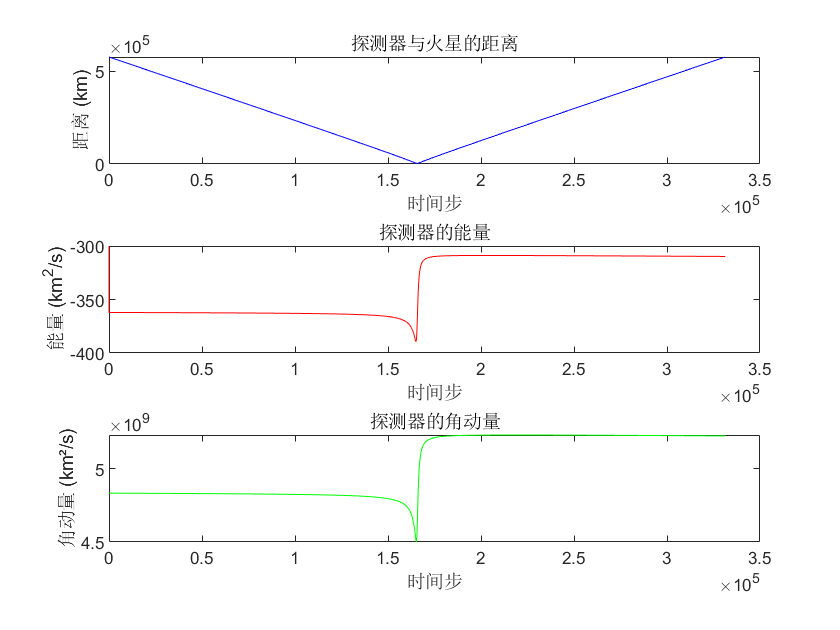
\includegraphics[width=0.8\textwidth]{images/parameter.png}
    \caption{探测器借力飞行期间参数变化图}
\end{figure}

探测器从远离火星的地方开始接近这颗红色星球,沿着双曲线轨迹逐渐靠近。在某个时刻,它抵达了近地点,随后又在火星引力的作用下逐渐远离。这一过程中,探测器经历了典型的双曲线轨道运动,进入火星的引力影响范围,在飞掠后被引力弹射出去,最终离开火星的影响球。

在接近火星时,探测器的总机械能出现短暂下降,随后在飞越火星后迅速回升并趋于稳定。这种能量变化反映了探测器与火星引力场的相互作用:当探测器靠近火星时,势能向动能转化,导致能量略微下降;而在飞越火星后,探测器的动能显著增加,总能量回升,表明它从火星引力场中“借”到了额外的能量,从而提升了轨道速度。

与此同时,探测器的角动量也经历了显著变化。在接近火星时,角动量略有下降,这是轨道方向逐渐调整的结果;而在飞越火星后,角动量迅速上升并趋于稳定。这种变化表明探测器在火星引力的作用下发生了轨道偏转,其运动方向发生了显著改变。

通过这次引力助推,探测器成功改变了自身的轨道能量和角动量。能量的增加使它获得了更高的轨道速度,而角动量的变化则导致轨道方向发生偏转。这种轨道调整不仅改变了探测器的飞行路径,还为其后续的深空探测任务提供了新的动力。例如,它可能利用这次引力助推前往更远的行星或小行星带,继续执行科学探测任务。

整个过程体现了引力助推的物理原理:探测器借助火星的引力场调整轨道,既节省了燃料,又实现了轨道能量和方向的优化。这种技术是深空探测任务中常见的策略,能够帮助探测器以更低的成本完成复杂的任务目标。

\begin{figure}[H]
    \centering
    \begin{subfigure}{0.45\textwidth}
        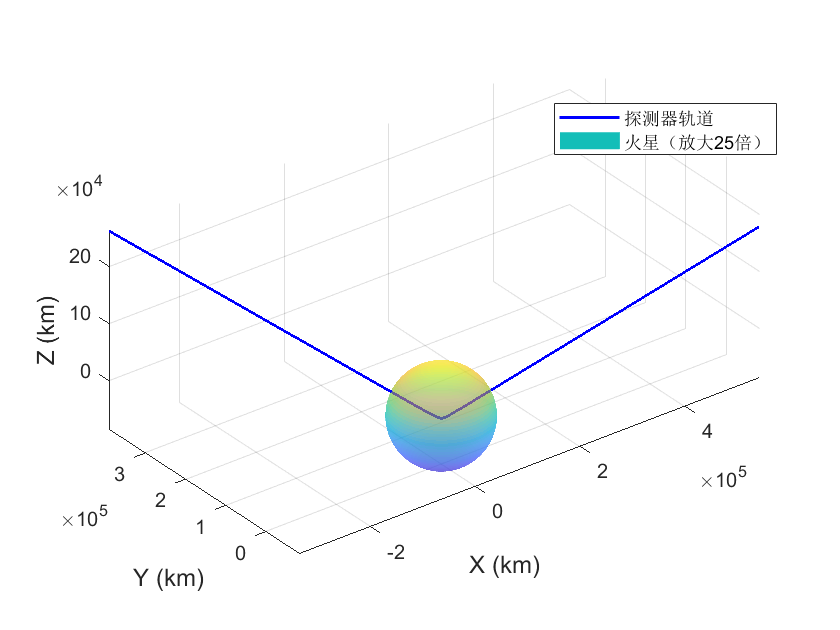
\includegraphics[width=\textwidth]{images/mars_orbit.png}
        \caption{实际轨道}
    \end{subfigure}
    \begin{subfigure}{0.45\textwidth}
        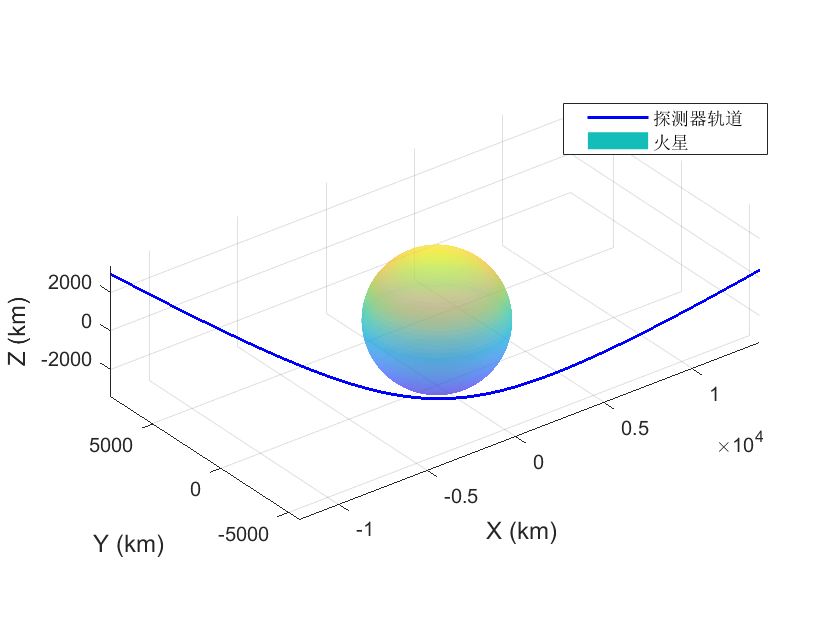
\includegraphics[width=\textwidth]{images/mars_orbit_zoom.png}
        \caption{局部放大}
    \end{subfigure}
    \caption{火心坐标系下探测器轨道图}
\end{figure}

\lstinputlisting[language=Matlab]{code/measure_deflection.m}

\subsection{日心坐标探测器、火星、地球飞行轨道}

\begin{figure}[H]
    \centering
    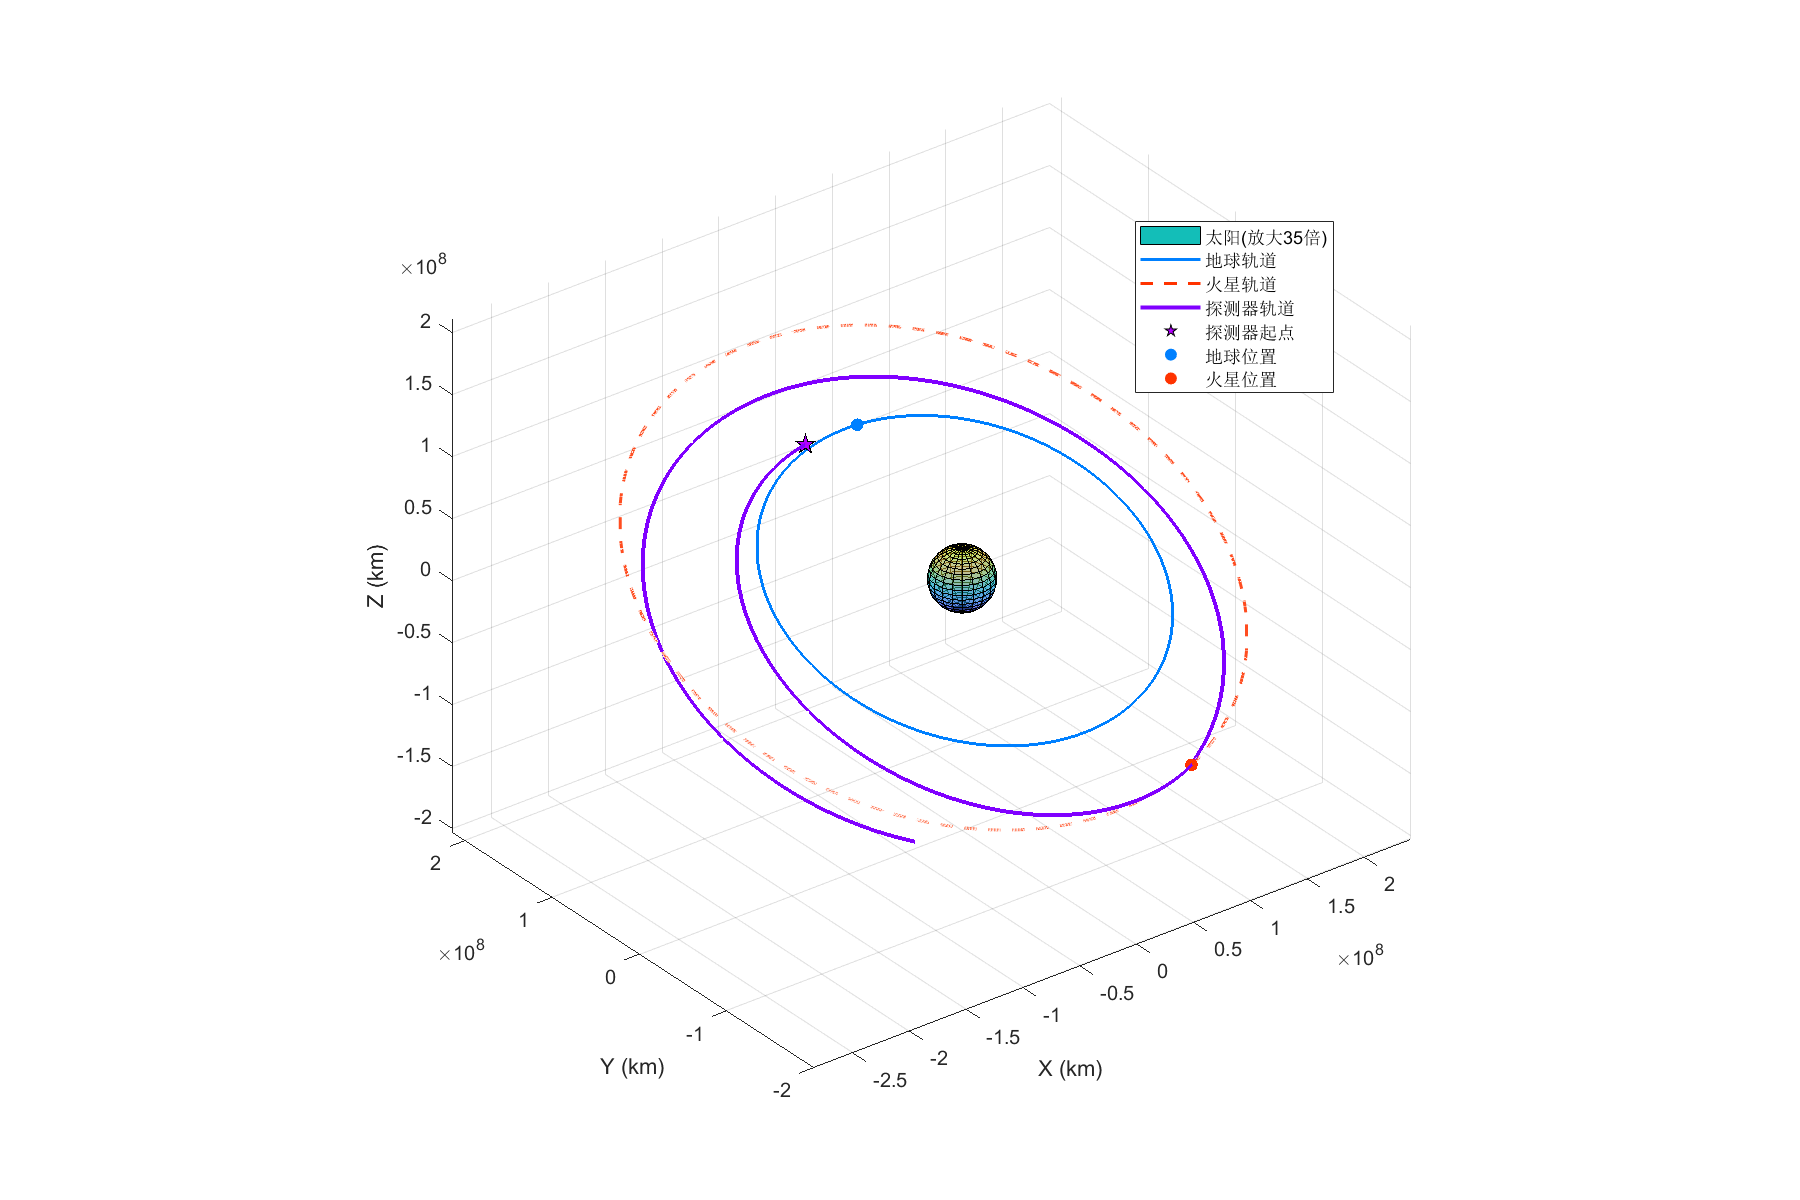
\includegraphics[width=0.8\textwidth]{images/solar.png}
    \caption{日心坐标系下探测器、火星、地球全程飞行轨道图}
\end{figure}

日心坐标系下探测器、火星和地球的飞行轨道图直观展示了天体运动轨迹。首先,地球轨道近乎圆形,体现了地球稳定的公转特性,轨道倾角接近0度,几乎在黄道面上运动,而火星轨道则位于地球轨道之外且更椭圆,其倾斜的轨道面相对于黄道面有一个小角度,这些特性共同决定了探测器的飞行路径与行星的相对位置关系。

探测器的轨道从地球出发,逐渐接近火星,在引力作用下发生偏转,轨道方向和形状发生显著变化,偏转角度和速度变化可通过轨道方向和密集程度判断,而能量变化则由轨道形状和大小反映。

轨道图在任务规划、轨道控制和科学研究中具有重要价值,它能帮助确定最佳发射窗口和飞行路径,评估轨道控制效果,并研究行星际引力环境和轨道动力学特性。

\end{document}